\documentclass[11pt,a4paper]{article}

\usepackage{longtable}
\newcommand \bt{\begin{longtable}{p{0.65\textwidth}p{0.25\textwidth}}}
\newcommand \et{\end{longtable}}
 
\usepackage[pdftex,usenames,dvipsnames]{color}
\usepackage{graphicx,psfig,epsfig}
\usepackage{epstopdf}

\definecolor{classbg}{rgb}{0.707,0.648,0.586}
\definecolor{fieldbg}{rgb}{0.363,0.641,0.746}
\definecolor{conbg}{rgb}{0.711,0.793,0.836}
\definecolor{descriptbg}{rgb}{0.848,0.918,0.953}

\usepackage[T1]{fontenc}
\renewcommand*\familydefault{\sfdefault}

\usepackage[hmargin=2.5cm,vmargin=2.5cm]{geometry}
\setlength{\parindent}{0.0\textwidth}

\begin{document}

\section*{Results from 1D random walk}
Experiment run on 10/6/2010 at 15.06\\\\\
\colorbox{descriptbg}{\large{Parameters}}
\bt
Number of moves in each walk&33\\
Number of walks &200\\
Probability of moving right &0.4\\
Probability of moving left &0.4
\et
\colorbox{descriptbg}{\large{Theoretical Values}}

\bt
expected distance travelled in 33 moves &0.00\\
expected mean square distance for 33 moves &26.40\\
\et
\colorbox{descriptbg}{\large{Measured Values}}
\bt
average distance travelled in 33 moves &  -0.04\\
average square distance for 33 moves & 23.46
\et
\colorbox{descriptbg}{\large{Visualisation of results}}
\begin{figure}[htbp]
\begin{center}
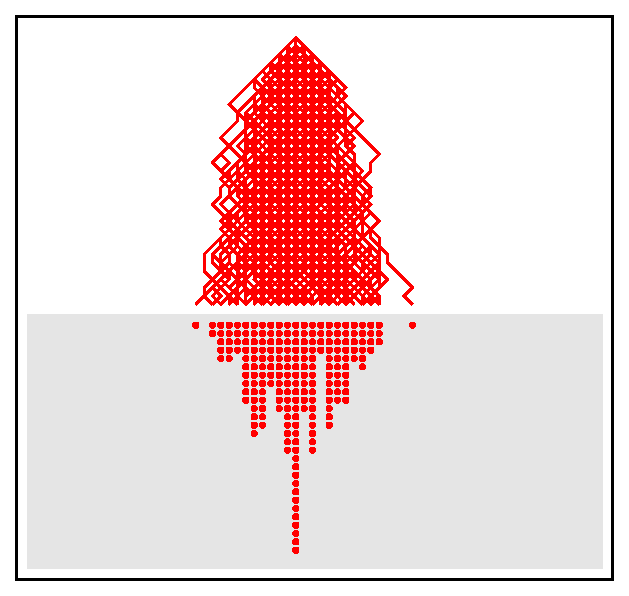
\includegraphics[width=0.8\textwidth]{CA33_R40L40.eps}
\caption{Upper panel shows cell pathways with vertical position representing timestep. 
Lower panel shows the distribution of final (horizontal) cell positions.}
\label{fig1}
\end{center}
\end{figure}


\end{document}
